\section{Data Collection and Transformation}

This section of the report will further discuss the application of the background research conducted into the extraction of wireless telemetry data (Section \ref{section:WirelessTelemetryResearch}) and the implementation of the system design (Section \ref{data_collection_design}). 
%Akshay to write these sections
\subsection{Data collection from the Router}
\label{Section: Data collection from the Router}

As discussed in previous sections all wireless telemetry data will be collected using the WiFi Radar feature on the ASUS Web GUI. There are multiple approaches to data collection which will be implemented and assessed in order to provide an efficient and non-intrusive method. As shown in Figure \ref{fig_WiFiRadar} the .db file can be downloaded through the ASUS GUI by clicking the "Save Database to File" button. The first two methods will implement data collection using Google Chrome as the main web driver and the final method will use SSH (Secure Shell) in order to access the router OS. 

\subsubsection{Tampermonkey Web Scraper} \label{section:Tampermonkey}

Tampermonkey \cite{tampermonkey} is a Google Chrome browser extension that enables the user to insert and use additional userscripts, which are JavaScript programs, into a web page. The addition of these userscripts allow the user to modify, add and automate functions on a web page. 

With Tampermonkey a userscript is to be created that periodically clicks the "Save Database to File" button. The script is configured to automatically start the data collection process once the specified web page is open (http://router.asus.com/configure.asp) so no additional setup is required. In the implementation of the script the HTML code was inspected to figure out the "input element id" of the buttons. The "Start Data Collection" and "Save Database to File" buttons have the element id's "startbutton" and "exportdbbtn" respectively. Then a function was written to click the "exportdbbtn" button every 5 seconds, which is in line with the lowest sampling interval for the ASUS router data recorder. The .db file is then downloaded into the directory specified in Google Chrome settings under Download Location, where it will go further processing (Section \ref{section:Data Extraction}).

\begin{lstlisting}[language=HTML, caption={Tampermonkey Data Collection Userscript Snippet}, label={lst:tampermonkey}]
(function start() {
    document.getElementById('startbutton').click();
})();

(function() {
    'use strict';
    var button = document.getElementById('exportdbbtn');
    setInterval(function(){
	button.click()
},5000)
})();
\end{lstlisting}




\subsubsection{Selenium WebDriver}

Selenium WebDriver is a web-based automation tool, the Python APIs allows for connection with a web browser of the users choice through which browser-based automation suites and tests can be easily created \cite{selenium}. In this project Selenium will be implemented to automate the data retrieval part of the telemetry pipeline, using the ASUS Web GUI. 

Firstly, the Selenium working environment has to be setup, for this the package and a web-driver must be installed. The Google ChromeDriver web-driver will be the main interface as it provides capabilities for automated testing of webapps, navigation of web pages, JavaScript execution and much more. ChromeDriver version 87.0.4280.88 is used as this is the version associated with the Google Chrome Browser pre-installed on the work station. Then using ChromeDriver a new window is opened in order to access the desired web page, which in this case is the ASUS router login page (http://router.asus.com/Main\_Login.asp) as shown in Figure \ref{fig:ASUSLoginPage}. From this point the \textit{find\_element\_by\_id()} function is used to identify the username and password elements on the web page in order to login to the router. 

\begin{lstlisting}[language=Python, caption={ASUS Router Login Code Snippet (Selenium)}, label={lst:selenium}]
login_user = driver.find_element_by_id('login_username')
login_user.send_keys(USERNAME)
login_pass = driver.find_element_by_name ('login_passwd')
login_pass.send_keys(PASSWORD)
\end{lstlisting}

\begin{figure}[ht]
    \centering
    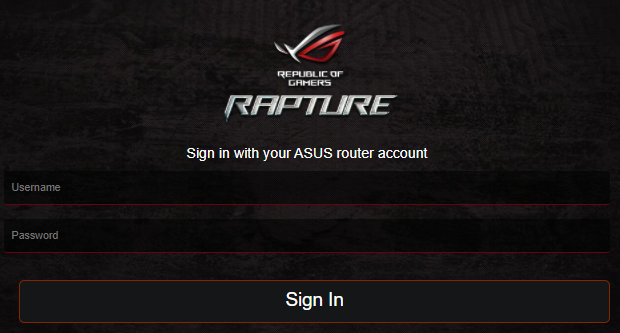
\includegraphics[width=1\linewidth]{pages/Chapter4/Chapter 4 Images/ASUSLoginPage.PNG}
    \caption{ASUS Web GUI Login Page}
    \label{fig:ASUSLoginPage}
\end{figure}

Now having logged into the ASUS router Web GUI, the next stage is to navigate into the Advanced Troubleshooting page (http://router.asus.com/configure.asp), which is where the data collection process is configured and from where the database file is downloaded. Then using the same procedure described in Section \ref{section:Tampermonkey}, the data collection process is started and the "exportdbbtn" is periodically clicked every 5 seconds using a \textit{while True} forever loop.

This method of data retrieval will automatically launch the ChromeDriver, login to the ASUS router Web GUi, navigate to the data collection configuration page and start the automatic download of the database file every 5 seconds. 


\subsubsection{Secure Shell (SSH)}

SSH is a network communication protocol that utilises encryption to secure the connection between client and server, allowing network service operations \cite{ssh}. For this project SSH will be used for remote command execution to login and retrieve the database file from the ASUS router. The SSHv2 protocol version is used, and was initially tested using the PuTTY client \cite{putty}. The standard TCP port for SSH is 22 but in the router setting this had to be changed to 1026 as the recommended SSH ports for the ASUS router was 1025 - 65535 due to security concerns. Having now established that it is possible to SSH into the ASUS router, the next step is to find where the database file is stored. Using the command \textit{ls} all directories were searched in order to find the file location of the database, Figure \ref{fig:PuttyAsusFiles} shows a non-exhaustive list of files and directories stored on the ASUS router. Further this, it was found that the database file location was \textit{'/tmp/db/visdata.db'}.

\begin{figure}[ht]
    \centering
    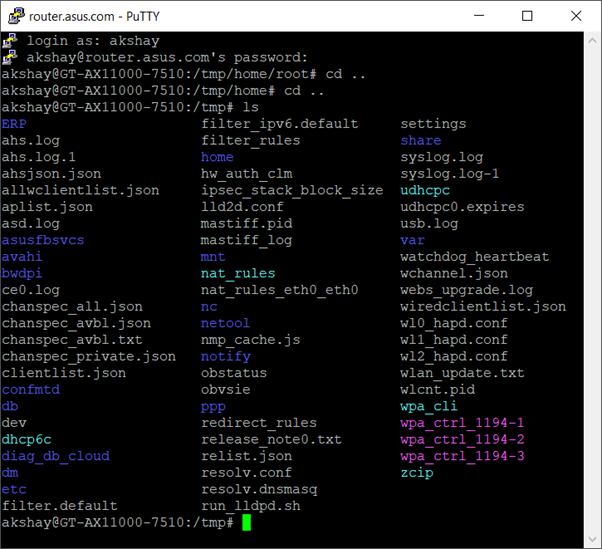
\includegraphics[width=1\linewidth]{pages/Chapter4/Chapter 4 Images/PuttyFiles.png}
    \caption{List of Computer Files on ASUS Router Using PuTTy}
    \label{fig:PuttyAsusFiles}
\end{figure}

Next a Python Script that would run in the background of the laptop connected to the ASUS router, needed to be created. To establish an SSH connection to the router the package Paramiko \cite{Paramiko} is used as this allows implementation of the SSHv2 protocol for Python.

\begin{lstlisting}[language=Python, caption={Paramiko SSH Client Python Code Snippet}, label={lst:paramiko}]
ssh_client = paramiko.SSHClient()
ssh_client.set_missing_host_key_policy(paramiko.AutoAddPolicy())
ssh_client.connect(host,port,username,password)
\end{lstlisting}

Then the SCP Python module \cite{scp} for Paramiko is used as this enables the transport of files between client and server via the SCP1 protocol. The SCPClient \textit{get.transport()} function is used to retrieve the database file every 5 seconds once again using a \textit{while True} loop.

\begin{lstlisting}[language=Python, caption={SCP Client Python Code Snippet For Data Retrieval}, label={lst:SCP}]
ssh_client.scp = SCPClient(ssh_client.get_transport())
while True:
    ssh_client.scp.get('/tmp/db/visdata.db', localpath)
    time.sleep(5)
\end{lstlisting}


\subsection{Data Extraction} \label{section:Data Extraction}

Now with the data retrieval section of the telemetry pipeline established, the next stage is to implement the data extraction process from the .db database file. As stated in Section \ref{Section: Data Categorisation} there are many data tables within the database files, a number of which are redundant in the progression of this project. Due to this only the ChannelStats, PacketRequested, Datathroughput, assocsta and PSRetry tables will be converted into the JSON format. 

\subsubsection{Detection of DB File}

With the aim of fully automating the data collection, retrieval and transformation portions of the wireless telemetry pipeline, and further the implementation of the data collection from the router (Section \ref{Section: Data collection from the Router}) there needs to be method for detecting when a new database file is downloaded. Once it has been detected that a new database file has been downloaded into a specified directory, the program should trigger the data transformation functions. 

The implementation of this automatic file detection is conducted using the Watchdog Python API library which allows the system to monitor for file system events \cite{watchdog}. The process of creating a file system monitor to detect changes in a directory is as follows. First, an handler instance of the \textit{watchdog.observers.Observer} thread class is created. Then, a subclass of the \textit{watchdog.events.FileSystemEventHandler} is created. Next, the directory path to be monitored is set and scheduled using the event handler attached to the observer instance. Finally, the observer thread is started where it will wait an event to trigger further processes. 

\begin{lstlisting}[language=Python, caption={Watchdog File System Event Handler Code Snippet}, label={lst:watchodog}]
class Handler(FileSystemEventHandler):
    @staticmethod
    def on_any_event(event):
        if event.is_directory:
            return None

        elif event.event_type == 'created':
            print ("Received created event - %s.")
            time.sleep(5)
            fileAdded()

        elif event.event_type == 'modified':
            print ("Received modified event - %s.")
\end{lstlisting}

As shown in the listing above when a new file is added to the directory being monitored, the funtion \textit{fileAdded()} is called. In this function the name of the latest file to be added is obtained using the Python modules glob and os. 

\begin{lstlisting}[language=Python, caption={Getting The Latest File Name Code Snippet}, label={lst:watchodog}]
def getLatestFileName():
    list_of_files = glob.glob('C:/Users/.../*.db')
    latest_file = max(list_of_files, key=os.path.getctime)
    return latest_file
\end{lstlisting}

Now having detected that a new database file has been downloaded, and with the name of the new file obtained, further data transformation process can be executed. 

\subsubsection{Data Extraction from DB File}

For the automation of the data extraction process a Python script is created that will open and read all relevant data in the .db file, then it will convert the data into Python objects and finally serialise these objects into the JSON format. 

In order to open and read in the .db file in Python the SQLite3 library is used, because it allows for access into databases that use nonstandard variants of the SQL query language \cite{sqlite3}. Firstly, a \textit{Connection object} is created to establish a connection to the SQLite database, where the object will represent the database \cite{sqlitePython1}. 

\begin{lstlisting}[language=Python, caption={SQLite3 Database Connection Object Code Snippet}, label={lst:Connection Object}]
def create_connection(db_file): 
    conn = None
    try:
        conn = sqlite3.connect(db_file) 
        return conn
    except Error as e:
        print(e)
    
    return conn
\end{lstlisting}

Having established the database connection, a cursor object is created (\textit{conn.cursor()}) so that its \textit{execute()} method can be called to perform SQL commands. Then a \textit{SELECT} statement is executed so as to access the data inside a specified datatable. Next, the method \textit{fetchall()} of the cursor object is called in order to retrieve all the data inside a datatable. 

\begin{lstlisting}[language=Python, caption={SQLite3 Cursor Object and Its Execute and Fetchall Method Code Snippet}, label={lst:Connection Object}]
cur = conn.cursor()
cur.execute("SELECT *FROM RxCRSGlitches")
rows = cur.fetchall()
\end{lstlisting}

With the .db database file now opened and with the ability to read data from it, the next step is to convert the datasets into Python Objects. For this each row in the datatable is temporarily stored into a tuple, which then gets appended into an array and this process is repeated for all rows in the table. Then, the Python object is serialised and converted into a JSON string using the \textit{json.dumps()} function. The \textit{dumps()} function is used rather than \textit{dump()} because the later writes Python serialised objects directly into a file, whereas the other encodes the object into a JSON formatted string. After this, the JSON formatted string is written into an outfile and saved into a specific directory to undergo further processing if required or to be directly uploaded onto the S3 Bucket. This process above is repeated and performed for every datatable that needs to be converted. 

Due to the fact that new datasets are appended to the .db database file even after downloading the latest version, in order to only have the latest timestamps and to avoid the use of very large JSON files a timestamp limit needs to be introduced. This is simply achieved using an if statement with a global cut off timestamp variable on the last datatable converted. 

\begin{lstlisting}[language=Python, caption={JSON Conversion Code Snippet}, label={lst:conversion example}]
rowarray_listassocsta = []
for row in rows:
    if row[1] > cutOffTimestamp:
        lastTimestamp = row[1]
        tupleassocsta = (row[0], row[1], row[2], row[3], row[4])
        rowarray_listassocsta.append(tupleassocsta)
            
stringassocsta = json.dumps(rowarray_listassocsta)

with open('C:/Users/...', 'w') as outfile:
    outfile.write(stringassocsta)
\end{lstlisting}

%Anurag here
\subsubsection{Data Compression of JSON Files}
\label{data_compression}
Once the data has been split up into 5 different JSON files after each relevant data table has been extracted. The python script in charge of compression works as shown by the block diagram in Figure \ref{fig:json_compression}. JSON files are retrieved and compressed into one JSON file for easier processing and transportation, while also removing any unnecessary data. It does this by retrieving each JSON file, generating a list of available MAC Addresses available and for each one, iterating through the data tables for 1 time stamp.
\begin{figure}[ht]
    \centering
    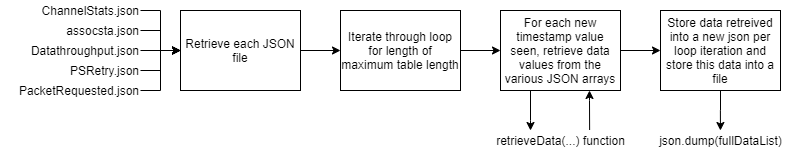
\includegraphics[width=1\linewidth]{pages/Chapter4/Chapter 4 Images/json_compression.png}
    \caption{Block Level Diagram of Compression Transformation of JSON Datafiles}
    \label{fig:json_compression}
\end{figure}
The diagram in Figure \ref{fig:data_table_data} shows what data can be retrieved from within each data table and how it appears within the new compressed JSON file. Only the most relevant and usable data is retrieved from each table, otherwise it removed.
\begin{figure}[ht]
    \centering
    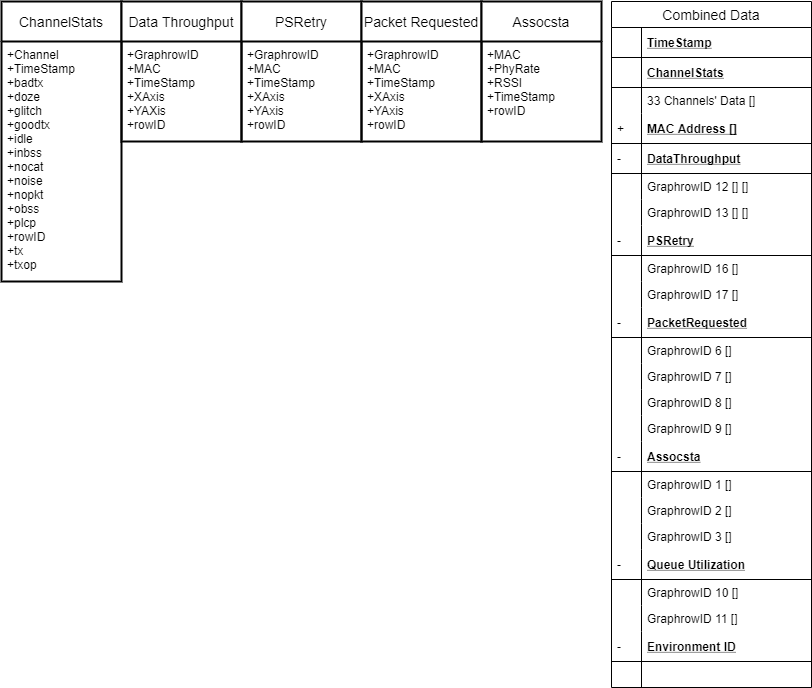
\includegraphics[width=1\linewidth]{pages/Chapter4/Chapter 4 Images/router_data-Dataset Contains.png}
    \caption{Relevant Data within each Data Table}
    \label{fig:data_table_data}
\end{figure}


\subsection{Telemetry Pipeline 1/3 - Upload to Cloud Directly}
The first pipeline method to be implemented is for the data to be taken from the laptop directly to the cloud. In this route an API Gateway is setup on the cloud as described in %\ref{}
and data can be sent to it for data to be sent and stored securely to an S3 bucket for pre-processing. The API Gateway follows the RESTful framework described in \ref{fig:api_gateway_methods}
%DON@T FORGET TO FINISH REFERENCE HERE TO API GATEWAY IMPL. SECTIOn



Using the Put method under the URL \textit{s3://gdp2020rawdata/\{timestamp\}/\{item\}} allows us to place the individual JSON files into the raw data bucket. Once all 5 JSON files are uploaded under the names:
\begin{itemize}
    \item \{timestamp\}\_PSRetry.json
    \item \{timestamp\}\_PacketRequested.json
    \item \{timestamp\}\_ChannelStats.json
    \item \{timestamp\}\_assocsta.json
    \item \{timestamp\}\_Datathroughput.json
\end{itemize}
Then an empty file is also uploaded to the cloud that also follows this pattern,\\ 
\textit{\{timestamp\}.complete}, which will trigger the pre-processing Lambda function. This process was previously described in \ref{cloud_lambda}. Once the Lambda function is triggered by this .complete file, will complete the transform function described above in Section \ref{data_compression} and will store the pre-processed data or \textit{compressed} data into the S3 Bucket as \\\textit{s3://gdp2020ppdata/compresseddata/\{timestamp\}.json}.

Using the Python \textit{requests} package \cite{python_requests_lib}, one can begin to upload as necessary using the following parameters:
\begin{itemize}
    \item \textbf{Payload}: json.dumps(JSON object)
    \item \textbf{Headers}:\begin{itemize}
        \item \textit{Content-Type}
        \item \textit{Host}
        \item \textit{Authorisation}
        \item \textit{Content-Length}
        \item \textit{Content-Type}
    \end{itemize}
\end{itemize}
After the requests payload is defined with the correct headers, using the following function in Listing \ref{lst:request_code} and storing the response, one can view the status code and use it to confirm correct upload. This follows standard HTTP status code guidelines, with a response of 200 being correct operation and other response code illustrating that something went wrong.
\begin{lstlisting}[language=Python, caption={Requests Library Usage}, label={lst:request_code}]
response = requests.request("PUT", url=payload, headers=headers)
print(response.status_code)
print(response.text)
\end{lstlisting}




